\documentclass[twocolumn]{article}
\setlength{\columnsep}{20pt}
%\usepackage{url}
%\usepackage{algorithmic}
\usepackage[a4paper]{geometry}
\usepackage{datetime}
\usepackage[font=small,labelfont=it]{caption}
\usepackage{graphicx}
% Use Times NR as font
\usepackage{lmodern}
\usepackage[T1]{fontenc}

\usepackage{float}

% Better tables
\usepackage{tabularx}
% to make beautiful tables
\usepackage{booktabs}

\usepackage{microtype}
\usepackage{amsmath}
\usepackage{subfigure}

% Letterspacing macros
\newcommand{\spacecaps}[1]{\textls[200]{\MakeUppercase{#1}}}
\newcommand{\spacesc}[1]{\textls[50]{\textsc{\MakeLowercase{#1}}}}

\title{\huge{\textbf{Study doc: feature representation}}\\ \normalsize \Large{how does the feature representation  effect the embedding space}}

\author{Fabian Gröger\\fabian.groeger@stud.hslu.ch}
\date{\today}

\begin{document}
\maketitle

\begin{abstract}
The experiment aims to show how the embedding space will change when using different feature representations.
\end{abstract}

\section{Introduction}
The purpose of the feature representation is to represent the audio in a more compact form than the raw audio. The feature representation further determines the input size for the model. There are a lot of different ways to represent the an audio file in a more compact form. One of the most popular representations is the MFCCs, which is heavily used in the audio domain. However in the recent years, the trend leads more towards using the log Mel spectrogram, which is very similar to the MFCCs, but by omitting the last step of the calculation. This experiment aims to find the optimal feature representation for the thesis.

\section{Hyperparameters}
The hyperparameters used for this experiment are shown in table \ref{tab:Hyperparameters}. The experiment will be conducted using a state of the art ResNet18 architecture on the DCASE dataset. The hyperparameters in section \textit{Feature representation} as well as the sample rate are the default ones proposed by the organisers of the DCASE challenge within the baseline project.
The optimal feature representation will be evaluated for \texttt{[LogMel, MFCCs]}.

\begin{table}[H]
    \centering
    \caption{Hyperparameters used for the experiment}
	\label{tab:Hyperparameters}
    \begin{tabular}{l|l}
        \toprule
        \textbf{Hyperparameter} & \textbf{value} \\ 
        \midrule[1pt]
        Dataset & DCASE \\
        \hline
        Model & ResNet18 \\ 
        \hline
        Epochs & 30-50 \\ 
        \hline
        Batch size & 128 \\ 
        \hline
        Optimizer & Adam \\ 
        \hline
        Learning rate & 1e-5 \\
        \hline
        Margin & 1.0 \\
        \hline
        L2 regularisation factor & 0.01 \\
        \hline
        Embedding dimension & 64 \\
        \hline
        Prefetch batches & Autotune (-1) \\ 
        \hline
        Random selection buffer & 64 \\ 
        \hline
        Shuffle dataset & True \\
        \hline
        Random seed & 1234 \\
        \midrule[1pt]
        \multicolumn{2}{l}{\textit{Multi threading}} \\
        \midrule[1pt]
        Number of generators & 16 \\ 
        \hline
        Number of parallel calls & 16 \\
        \midrule[1pt]
        \multicolumn{2}{l}{\textit{Audio sample}} \\
        \midrule[1pt]
        Sample rate & 16000 \\ 
        \hline
        Sample size & 10 \\
        \hline
        Sample tile size & 5 \\
        \hline
        Sample tile range & 5 \\
        \hline
        Convert to mono & True \\
        \midrule[1pt]
        \multicolumn{2}{l}{\textit{Feature representation}} \\
        \midrule[1pt]
        Feature extractor & \textbf{[LogMel, MFCCs]} \\ 
        \hline
        Frame length & 480 \\
        \hline
        Frame step & 160 \\
        \hline
        FFT size & 1024 \\
        \hline
        Number of Mel bins & 128 \\
        \hline
        Number of MFCC bins & 13 \\
        \bottomrule
    \end{tabular}
\end{table}

\begin{figure}[t]
\centering
    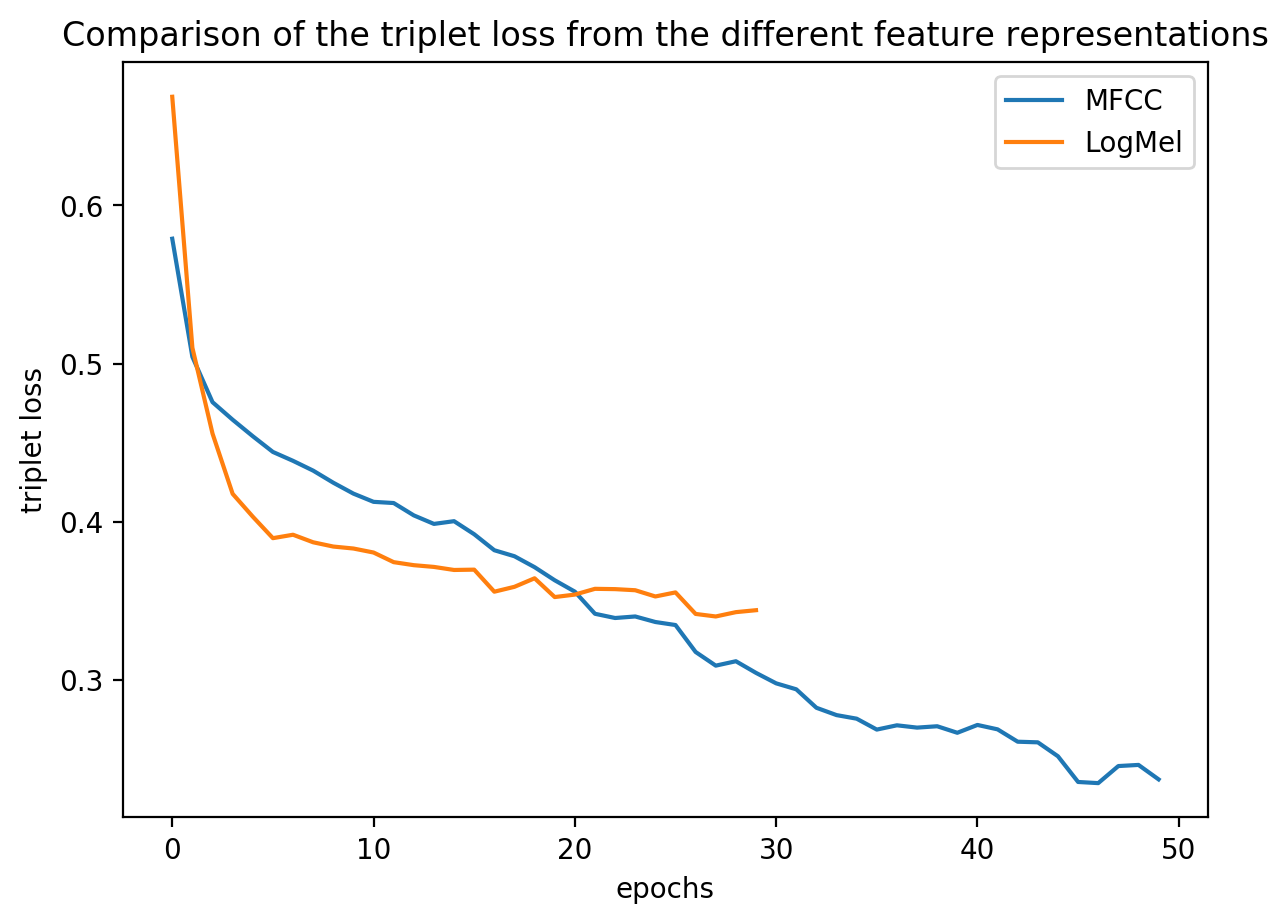
\includegraphics[width=\linewidth]{assets/triplet_loss_feature_representation.png}
    \caption{Plot of the triplet loss of the different feature representations}
    \label{fig:plot-triplet-loss-feature-representations}
\end{figure}

\section{Results}
Comparing the effect of different regularisation factors on the embedding space is pretty hard, since comparing embedding spaces is not very straight forward and is a rather tricky task. This is mainly because of the fact, that to visualise the high dimensional embedding space in a way humans can perceive it, it has to be reduced to two or three dimensions. Therefore the original space can not be examined, and the visual representation is always an approximation of the space in a lower dimension. To still compare the feature representations, a simple logistic classifier is trained on top of the resulting embedding spaces, which aims to show how well a simple classifier works with the embedding space. This will show how good the resulting embedding space is. The classifier is trained for 40 epochs with the same parameters as the embedding model (table \ref{tab:Hyperparameters}).

Figure \ref{fig:plot-triplet-loss-feature-representations} shows the difference between the triplet loss from the model using the different feature representations. It shows that the model trained using the MFCCs results in a significantly lower loss than the model using the log Mel spectrogram. The model using the log Mel spectrogram seem already converging at epoch 30.

Figure \ref{fig:classifier-f1-feature-represenations} shows the different F1 scores of the logistic classifier, which is trained using the embedding space as input. This provides an idea of how well the embedding space separates the classes and therefore gives a performance gain. The figure \ref{fig:classifier-f1-feature-represenations} shows clearly that the classifier trained on top of the log Mel spectrogram reached a higher F1 score. The metric further shows, that the classifier using the MFCCs embedding space fails to improve the F1 score over time, whereas the classifier for the log Mel spectrogram shows a definite increase over time.

\begin{figure}[t]
\centering
    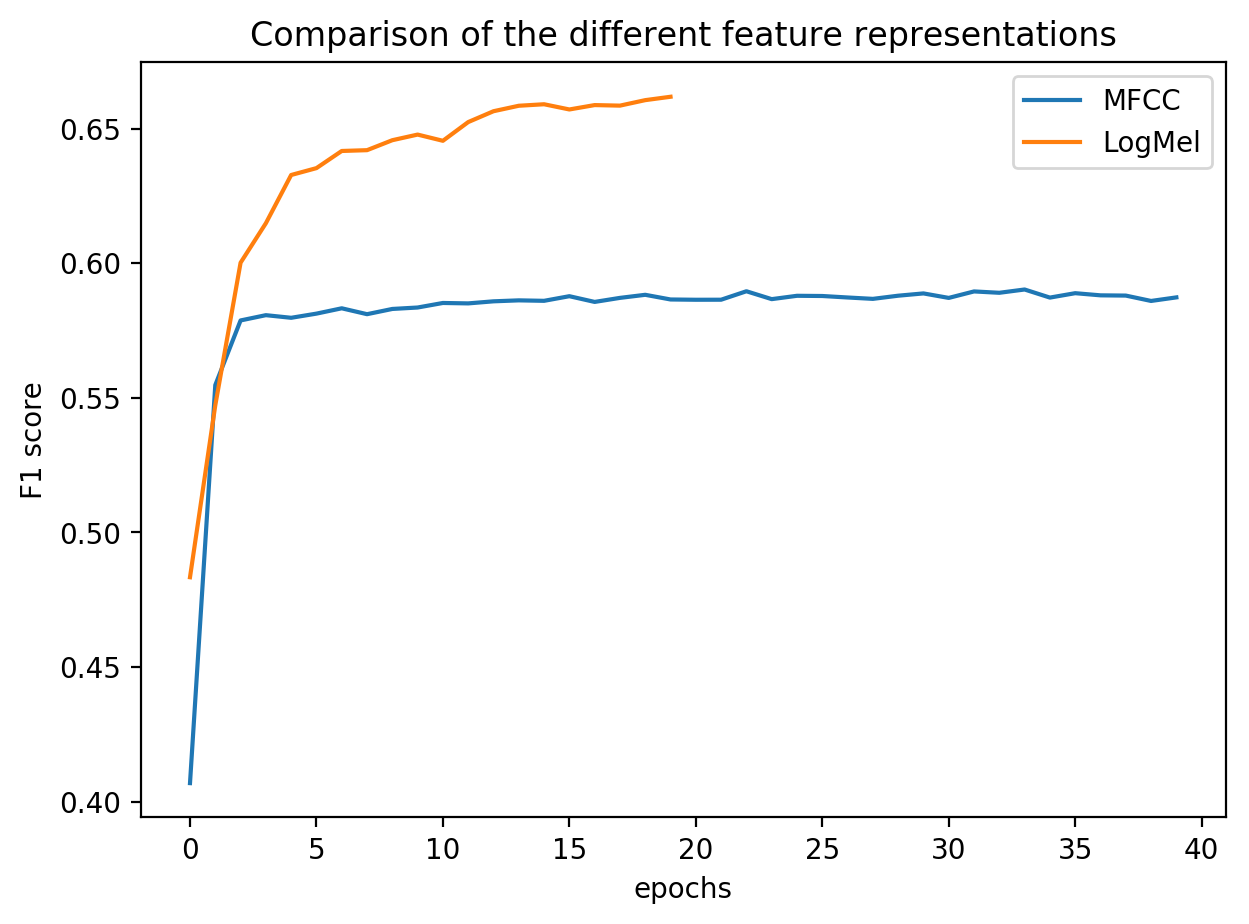
\includegraphics[width=\linewidth]{assets/f1_feature_representation.png}
    \caption{F1 score of the trained classifier using the trained embedding spaces from the different feature representations}
    \label{fig:classifier-f1-feature-represenations}
\end{figure}

\section{Conclusion}
From figure \ref{fig:plot-triplet-loss-feature-representations} it seems that the optimal feature representation is the MFCCs since it reached a significantly lower loss value. It further shows that the model would be able to benefit from further training since the model is still decreasing. However, when looking at the resulting F1 score of the classifiers (figure \ref{fig:classifier-f1-feature-represenations}), the result shows, that even though the MFCCs representation reached a lower triplet loss, the classifier fails to separate the resulting clusters using a hyperplane. 

This experiment shows that the optimal feature representation for the current thesis is using the log Mel spectrogram, since it resulted in a higher F1 score of the classifier, even though the triplet loss value is higher than the one using the MFCCs. 

This is mainly due to the different nature of the feature representations. The MFCCs representation input size (498, 13) is significantly lower than the log Mel spectrogram representation input size (498, 128). The MFCCs is a more compact representation, which seems to have a negative effect on the model's performance.

This experiment shows that the model benefits from using a representation which has more features and therefore, the log Mel spectrogram is used as the optimal representation for the thesis.

\section{Next steps}

For the next experiments, the feature representation log Mel spectrogram is chosen.

\end{document}